\chapter{Discovering (Setting Limit for) \Bmumumu at LHCb}
\label{chap:sel}

\textit{LHCb's flagship analyses contain several muons in the final state coming from differently flavoured $B$ mesons. Despite being in this category, search for \Bmumumu is limited by the rareness of its occurrence as well as different backgrounds that can mimic its signature in the detector. Moreover, presence of invisible neutrino does induce uncertainties into reconstruction. This \autoref{chap:sel} will concentrate on characterisation of backgrounds as well as selection that is performed in order to reduce the backgrounds.}


\section{Topology of at LHCb \Bmumumu at LHCb}

Upon hadronisation of $b\bar{b}$ pair \Bpm particle will travel less than a millimetre in the laboratory frame of reference before it decays into its decay products. This allows reconstruction of a primary vertex \Gls{PV} and its decay vertex, \textit{secondary vertex} \Gls{SV}. By joining these vertices, direction as well as length of the \Bpm existence, also known as flight distance (\Gls{FD}), can be established. In order to infer information about kinematic properties of \Bpm, the decay products are studied. All three muons are used to reconstruct the visible four-momentum. By conservation of momentum with respects to the direction of the flight of \Bpm, neutrino is assigned all missing momentum transverse to the direction of the flight of \Bpm. The schematic diagram can be seen in \autoref{fig:sigtopolog}.

\begin{figure}[!h]
	\centering
	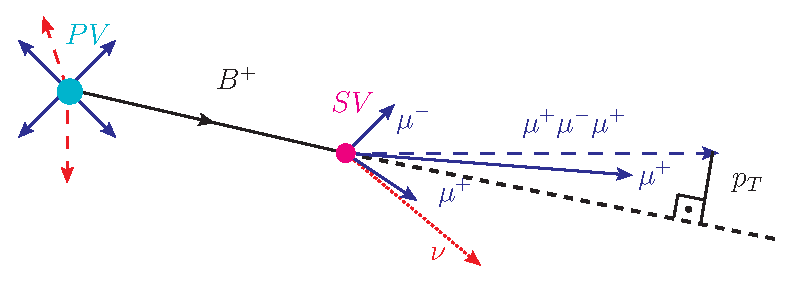
\includegraphics[width = 0.8\textwidth]{figs/sel/DecReco_fin.eps}
	\caption{Schematic view of \Bmumumu decay. At $pp$ interaction point, or $PV$, $b\bar{b}$ pair hadronizes into \Bpm. \Bpm flies some distance before decaying into three muons and neutrino. All charged tracks (in filled-blue) seen can be combined into four-vector representing the visible part of the decay (semi filled-blue). Information about invisible neutrino (semi filled-red) are deduced from the conservation of momentum with respect to the direction of the flight of \Bpm. Neglecting momentum component parallel to the direction of flight for neutrino, transverse component of momentum is given.}
	\label{fig:sigtopolog}
\end{figure}

Altogether it allows for reconstruction of a quantity, \textit{corrected mass}, that plays similar role to invariant mass in fully reconstructed decays. Invariant mass is usually used in \Gls{LHCb} for fitting distribution from which physics results are extracted as it distinguishes well signal from background and there is minimal modelling problem.

\textit{Corrected mass} is defined as

\begin{equation}
	M_{corr} = \sqrt{{M}^{2} + |p^{2}_{T}|} + |p_{T}|,
\end{equation}	
where the $M^{2}$ is the invariant visible mass squared and $p^{2}_{T}$ is the missing momentum squared transverse to the direction of $B^{+}$ flight.

%\begin{equation}
%M_{B_{corr}} = \sqrt{M_{\mu^{+} \mu^{-} \mu^{+}}^{2} + |p_{T}|} + |p_{T}|,
%\end{equation}	

$M_{corr}$ can be thought of as the minimal correction to the visible mass to account for the missing neutrino information. The resolution on the \textit{corrected mass} hence becomes a critical quantity that needs to be understood. As the method of reconstruction of corrected mass relies heavily on the knowledge of \Bpm flight direction, the resolution of \Gls{PV} position and \Gls{SV} vertex is crucial. Let $\vec{{x}}_{PV}=\{x_{PV},y_{PV},z_{PV}\}$, $\vec{{x}}_{SV}=\{x_{SV},y_{SV},z_{SV}\} $ be \Gls{PV} and \Gls{SV} vertex position and $\vec{p}=\{p_{x},p_{y},p_{z}\}$ be the visible trimuon momentum. Then the missing transverse momentum to the direction of the flight $p_{T}$ (momentum of the neutrino) is


\begin{equation}
	p^{2}_{T} = |\vec{p} - (\vec{{x}}_{SV}-\vec{{x}}_{PV})\frac{\vec{p} \cdot(\vec{{x}}_{SV}-\vec{{x}}_{PV})}{|(\vec{{x}}_{SV}-\vec{{x}}_{PV})|^{2}}|^{2}
\end{equation}

In general in order to propagate error on $f(x,y,z)$, where $x,y,z$ are independent variables, the variance of $f(x,y,z)$

\begin{equation}
\begin{aligned}
	\langle f^{2}-\langle f \rangle^{2} \rangle  &=  \langle f(x+\delta x, y+\delta y, z+\delta z)^{2} - f(\langle x \rangle, \langle y \rangle, \langle z \rangle)^{2} \rangle \\
\end{aligned}
\end{equation}

Using first order Taylor expansion of variance and rewriting into the matrix form:

\begin{equation}
\begin{aligned}
%	\langle \frac{\partial{f}}{\partial{x}}  \frac{\partial{f}}{\partial{x}} \times \delta x^{2} + \frac{\partial{f}}{\partial{y}}  \frac{\partial{f}}{\partial{y}} \times \delta y^{2} + \frac{\partial{f}}{\partial{z}}  \frac{\partial{f}}{\partial{z}} \times \delta z^{2} + \sum_{i,j=1..3, i \neq j} \partial_{d_{i}} \partial_{d_{i}}  \frac{\partial{f}}{\partial{x}} \frac{\partial{f}}{\partial{y}} \rangle \\ 
%        = 
       \begin{bmatrix}
		\frac{\partial{f}}{\partial{x}} & \frac{\partial{f}}{\partial{y}} & \frac{\partial{f}}{\partial{z}} \\
       \end{bmatrix}
       \begin{bmatrix}
	       {\delta x}^{2} & \delta x \delta y & \delta x \delta z  \\ 
	        \delta y \delta x & {\delta y}^{2} & \delta y \delta z  \\
	        \delta z \delta x & \delta z \delta y & {\delta z}^{2}  \\
       \end{bmatrix}
       \begin{bmatrix}
		\frac{\partial{f}}{\partial{x}} \\ \frac{\partial{f}}{\partial{y}} \\\frac{\partial{f}}{\partial{z}} \\
       \end{bmatrix}
\end{aligned}
\end{equation}

So now assuming that $x=\vec{{x}}_{PV}$, $y=\vec{{x}}_{SV}$ and $z=\mathbold{\vec{p}}=\{E,p_{x},p_{y},p_{z}\}$,

\begin{equation}
\begin{aligned}
       \nabla^{T}_{x_{PV}} \rm{COV_{x_{PV}}} \nabla_{x_{PV}} + \nabla^{T}_{x_{SV}} \rm{COV_{x_{SV}}} \nabla_{x_{SV}} + \nabla^{T}_{p} \rm{COV_{p}} \nabla_{p}
\end{aligned}
\end{equation}

where \rm{COV} is the covariance matrix.

In conclusion in order to calculate error on \textit{corrected mass}, $\delta_{corrm}$


\begin{equation}
\begin{aligned}
	\delta_{corrm} = \sqrt{ \langle f^{2}-\langle f \rangle^{2} \rangle} = \sqrt{\nabla^{T}_{x_{PV}} \rm{COV_{x_{PV}}} \nabla_{x_{PV}} + \nabla^{T}_{x_{SV}} \rm{COV_{x_{SV}}} \nabla_{x_{SV}} + \nabla^{T}_{p} \rm{COV_{p}} \nabla_{p}} 
\end{aligned}
\end{equation}

which can be calculated analytically (method used for all the plots) or using numerical approximation of first derivative of \textit{finite differences}.

\section{Sources of Backgrounds}
The largest background that can be will be looking similar to signal comes from \textit{cascade decays}, where semileptonic $b \rightarrow c \rightarrow s$ or ($\bar{b} \rightarrow \bar{c} \rightarrow \bar{s}$) transition occurs. A typical example of this background in hadronic terms is $B^{+} \rightarrow (\bar{D}^{0} \rightarrow (K^{+} \rightarrow \mu^{-} \nu) \mu^{+} \nu$), where $K^{+}$ is misidentified as muon. Because $K^{+}$ is misidentified as muon, this type of background is denoted as misID background.

In fact, any other particle species that is misidentified, belongs to the misID background category. If the sign of the misidentified particle agrees with the sign of the mother \Bpm, it belongs to the same sign misID background (\textit{SS misID}) background. In the event where opposite sign particle to the mother \Bpm is misidentified, this background will be referred to as (\textit{OS misID}) background. However, \textit{OS misID} background is expected to have smaller rate as the misidentified particle would have to proceed via decays with additional particles or if coming as product from other $b$ hadronization.

The presence of other \B-hadron from $b\bar{b}$ pair does create its own decay chain and hence it is possible to combine one of its muon tracks with two muons from the "signal" \B. This is denoted as combinatorial background.

Then presence of neutrino in a final state allows for certain uncertainty regarding the information of the fourth decay product. If some of the tracks of the decays are not reconstructed, either because they are neutral, or either they are charged but they are soft, it means that the missing information may be attributed to the neutrino. \textit{Missing tracks} will hence create partially reconstructed background. Some of the most dangerous are ${B^{+} \rightarrow D \mu^{+} \nu}$ type partially reconstructed backgrounds where $B^+ \rightarrow (D^0 \rightarrow K^- \pi^+ \mu^{+} \mu^{-})\mu \nu$, where $\mathcal{B}(D^0 \rightarrow K \pi^+ \mu^{+} \mu^{-}) \approx 4.17\times 10^{-6}$ and $B^{+} \rightarrow D^0 \mu \nu \approx 10 \%$. This predicts $\mathcal{B}(B^+ \rightarrow K^+ \pi^- \mu^+ \mu^{-} ) = 1\times10^{-7}$.

\section{Analysis strategy}
\label{Strategy}

The analysis of the $B^{+} \rightarrow \mu^{+} \mu^{-} \mu^{+} \nu_\mu$ decay is divided into several different parts; signal selection, optimisation, normalisation, fitting and limit setting. Throughout this document, charge conjugates of the decays are assumed unless stated otherwise. Results presented are based on the analysis of the full 3 fb$^{-1}$ Run 1 dataset as well $\approx$ 1.7 fb$^{-1}$ Run 2 data (not using 2015 dataset due to very low sensitivity (high muon trigger thresholds)). Additionally the search will be conducted in a particular min$q^{2}$ = min($q^{2}(\mu_{1}^{+},\mu^{-}), q^2(\mu^{-},\mu_{2}^{+})$) region.
\newline To perform the search for $B^{+} \rightarrow \mu^{+} \mu^{-} \mu^{+} \nu_\mu$, a specific preselection was applied to form potential signal candidates. To reconstruct the mass of the $B^{+}$ with missing information about the neutrino, a corrected mass variable $M_{B_{corr}} = \sqrt{M_{3\mu}^{2} + |p^{2}_{\perp}|} + |p_{\perp}|$, where $M_{3\mu}^{2}$ is the invariant visible mass squared and $p^{2}_{\perp}$ is the missing momentum squared transverse to the direction of flight of $B^{+}$, is introduced. A simulation sample that mimics the decay of the $B^{+} \rightarrow \mu^{+} \mu^{-} \mu^{+} \nu_\mu$ passing through preseletion was used to develop further discriminating selection. To get the selection efficiency for different types of backgrounds, different proxy samples are used. For more details about samples used see Section~\ref{Data}.
\newline Combinatorial background, which arises as random combinations of tracks passing the preselection, is taken from the upper corrected $\mu^{+} \mu^{-} \mu^{+}$ mass side band, $M_{Bcorr} > 5.5$ GeV, where very few signal candidates are expected.

\section{Preselection for \Bmumumu}

Set of initial identification for signal \Bmumumu summarized in \autoref{tab:stripcutsB}, also known as \textit{stripping} selection was develloped in order to improve signal to background ratio. 

Firstly, all three muon tracks are required to have a significant \Gls{IP} with respect to the primary vertex. Minimum Impact Parameter $\chi^{2}$, (\Gls{minipchi2}), gives the minimum significance of a particles's trajectory to the primary vertex. Hence by requiring \Gls{minipchi2}$>9$ for muons is consistent with the hypothesis that the muon is $3\sigma$ away from the primary vertex and hence can be well differentiated. This selection suppresses prompt backgrounds. 

Each muon track is required to have good track $\chi^{2}$ per number of degrees of freedom (\texttt{ndof}) of the fit as well as certain low \Gls{pgh2}. This removes spurious tracks as well as tracks with low quality.

Each muon candidate is also identified with initial basic \Gls{PID} variables. Firstly muons are chosen due to their signature in the muons stations with the binary \texttt{isMuon} decision. Secondly, muons candidates are chosen such that it is more likely that the candidate is muon than pion or kaon using global DLLmu variables defined in \autoref{muonID}. This reduces the background from misidentified muons. 

\textbf{Corrected mass of $\boldsymbol{B^{+}}$ meson}, $M_{B_{corr}}$ - This is corrected mass of $B^{+}$ meson, using the corrected mass technique (see subsection 4.1.1) to correct for missing daughter information.
\newline\textbf{Flight distance} is the distance between primary vertex ($B^{+}$ production vertex) and secondary vertex ($B^{+}$ decay vertex). 
\newline\textbf{Flight distance $\boldsymbol{\chi^{2}}$} computes the significance of the flight distance between primary vertex and decay vertex of the $B^{+}$.
\newline\textbf{Direction angle cos($\boldsymbol{\theta_{B}}$)} is the cosine of the angle between the momentum vector of the $B^{+}$ meson and the direction of the flight of the $B^{+}$ meson from its primary vertex to its secondary vertex. Requiring cos($\theta_{B}$) close to unity translates into a well reconstructed event.  
\newline\textbf{Vertex $\boldsymbol{\chi^{2}}$ per degree of freedom} computes the $\chi^{2}$ of the vertex fit. Imposing upper band on this variable forces the tracks of the daughter particles to originate from the same point in the space.
\newline\textbf{Impact parameter}, \textit{IP}, is the shortest distance of approach of the track of the particle to the primary vertex. Since $B^{+}$ originates at the primary vertex, the extrapolated track of the $B^{+}$ should point close to the primary vertex, hence, the \textit{IP} is small. However, since the $B^{+}$ is long-lived the direction of the tracks of muons from the $B^{+}$ decay are different and hence the $IP$ tend to be much be bigger.
\newline\textbf{ Minimum Impact Parameter $\boldsymbol{\chi^{2}}$}, $\chi^{2}_{minIP}$, gives the minimum significance of a particles's trajectory to the primary vertex. Requiring $\chi^{2}_{minIP}>9$ for muons is consistent with the hypothesis that the muon is $3\sigma$ away from the primary vertex and hence can be well differentiated.
\newline\textbf{Delta-Log-likelihood for $\boldsymbol{x}$}, PID${x}$, calculates delta-log-likelihood of particle to be of type $x$ with respect to the pion hypothesis,
\begin{equation}
\Delta ln\mathcal{L}_{x\pi} =  ln(\mathcal{L}_{x})-ln(\mathcal{L}_{\pi}).
\end{equation}
The likelihood of identifying particle is inferred from PID information obtained from  different subdetectors. For a hadron, the likelihood is following:
\begin{equation}
\mathcal{L}_{x} = \mathcal{L}_{x}^{RICH} + \mathcal{L}_{x}^{CALO} + \mathcal{L}_{x}^{MUON},
\end{equation}
where $\mathcal{L}_{x}^{RICH}$ is the likelihood of particle to be of type $x$ given the information by RICH detector, $\mathcal{L}_{x}^{CALO}$ provides this information using the calorimeter output and $\mathcal{L}_{x}^{MUON}$ calculates the likelihood based on the information from muon stations. 
\newline\textbf{Track $\boldsymbol{\chi^{2}}$ per degree of freedom}, ${\chi^{2}_{tr}/dof}$, calculates the track $\chi^{2}$  per number of degrees of freedom of the
track fit.
\newline\textbf{Ghost probability} $P_{ghost}$ calculates the probability of misreconstruction of the track, where for each track 0 is most signal-like and 1 is most ghost-like. A charged particle is not considered to be a ghost if 70\% of the hits match between the reconstructed and simulated true tracks. Similarly, neutral particles are ghosts if simulated particle contributes less than 50\% of the reconstructed cluster energy from calorimeter.



\begin{table}%[H]
\begin{center}
\begin{tabular}{l|c l }

    \hline
     Candidate & Stripping Selection \\ \hline

	muon & $\chi^{2}_{minIP} > 9$ &  \rdelim\}{3}{1cm}[\ track] \\
	muon & $P_{T} >$ 0 \\
	muon & $\chi^{2}_{tr}/\rm{dof} < 3$ \\

	
	muon & $\Delta LL(\mu - \pi) > 0$ & \rdelim\}{3}{1cm}[\ \Gls{PID}] \\
	muon & $\Delta LL(\mu - K) > 0$ \\
	muon &  \texttt{isMuon==true} \\ \hline
	
	combination & $cos(\theta_{B}) >$ 0.999 \\
        combination & $p_{T} >$ 2000 \mev\\
	combination & $\chi^{2}_{FD} >$ 50\\
	combination & $\chi^{2}/\rm{dof} < 4$ \\
	combination & $0\ \mevcc\ <\ M_B\ <\ 7500\ \mevcc$ \\
	combination & $2500\ \mevcc\ <\ M_{B_{corr}}\ <\ 10000\ \mevcc $\\ \hline
     \end{tabular}

\end{center}
	\caption{Selection of events based on muon and the $B^{+}$ candidate requirements. \textit{Stripping selection} for the signal decay $B^{+} \rightarrow \mu^{+} \mu^{-} \mu^{+} \nu_\mu$ is the same for both Run1 and 2016 data.}
\label{tab:stripcutsB}
\end{table}



